\documentclass{beamer}

\usepackage[utf8]{inputenc}
\usepackage{graphicx}

\usepackage{biblatex}
\addbibresource[]{week08.bib}

\title{FIT2102 PASS - Week 8}
\author{Nicholas Cheng}

\begin{document}

\begin{frame}
    \titlepage
\end{frame}

\begin{frame}
    \tableofcontents
\end{frame}

% General function application

\section{Function application}
\begin{frame}
    \frametitle{\insertsection}
    \centerline{
        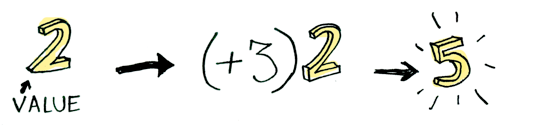
\includegraphics[scale=0.5]{images/value_apply.png}
    }
\end{frame}


% Functors

\section{Functors}

\begin{frame}
    \frametitle{\insertsection}
    The \textbf{main} difference now is that values are inside of a \textit{context}.
    \centerline{
        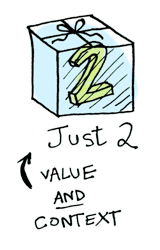
\includegraphics[scale=0.5]{images/value_and_context.png}
    }
\end{frame}

\begin{frame}
    \frametitle{\insertsection}
    Does this make a difference?
    \textbf{Yes}, but \textbf{no}.
    Lemme explain.
\end{frame}

\begin{frame}
    \frametitle{\insertsection}
    Ideally, we'd want something that does this.
    \centerline{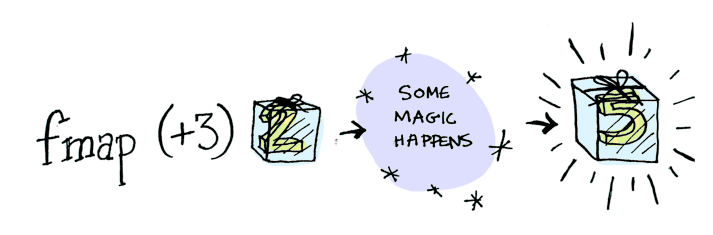
\includegraphics[scale=0.4]{images/fmap_apply.png}}
\end{frame}

\begin{frame}
    \frametitle{\insertsection}
    \framesubtitle{What the fmap?!}
    \centerline{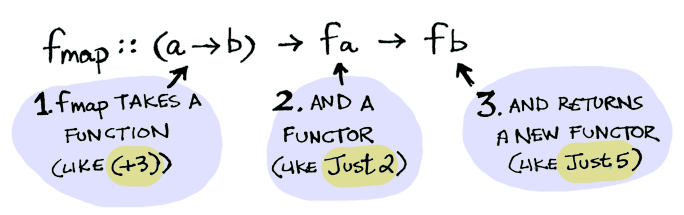
\includegraphics[scale=0.4]{images/fmap_def.png}}
\end{frame}

\begin{frame}
    \frametitle{\insertsection}
    \framesubtitle{Stop wasting my time and just tell me what to do!}
    \centerline{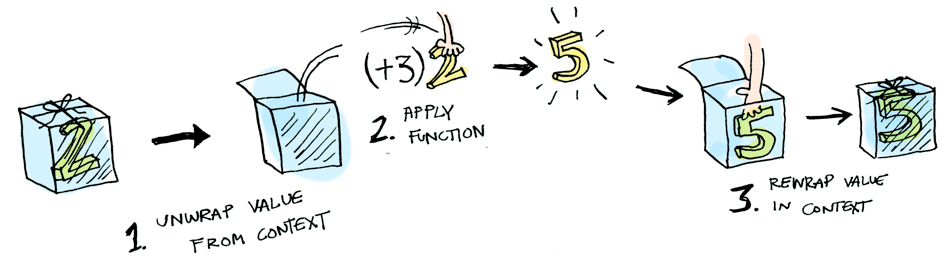
\includegraphics[scale=0.3]{images/fmap_just.png}}
    Say, this looks awfully familiar.
\end{frame}

\begin{frame}
    \frametitle{\insertsection}
    \centerline{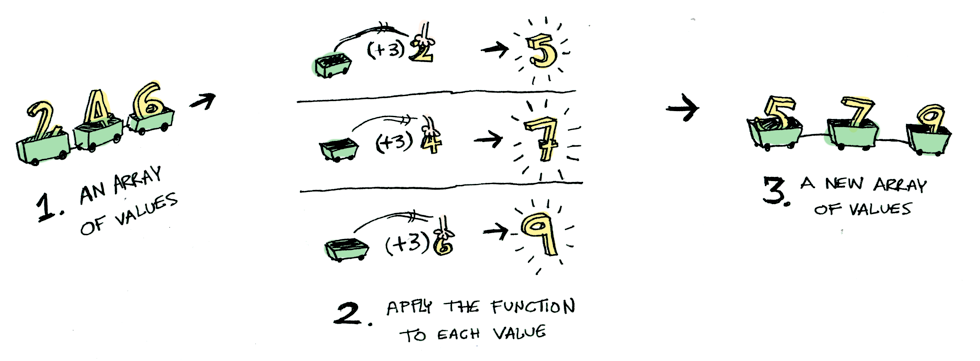
\includegraphics[scale=0.3]{images/fmap_list.png}}
    And lists too?
\end{frame}

\begin{frame}
    \frametitle{\insertsection}
    \centerline{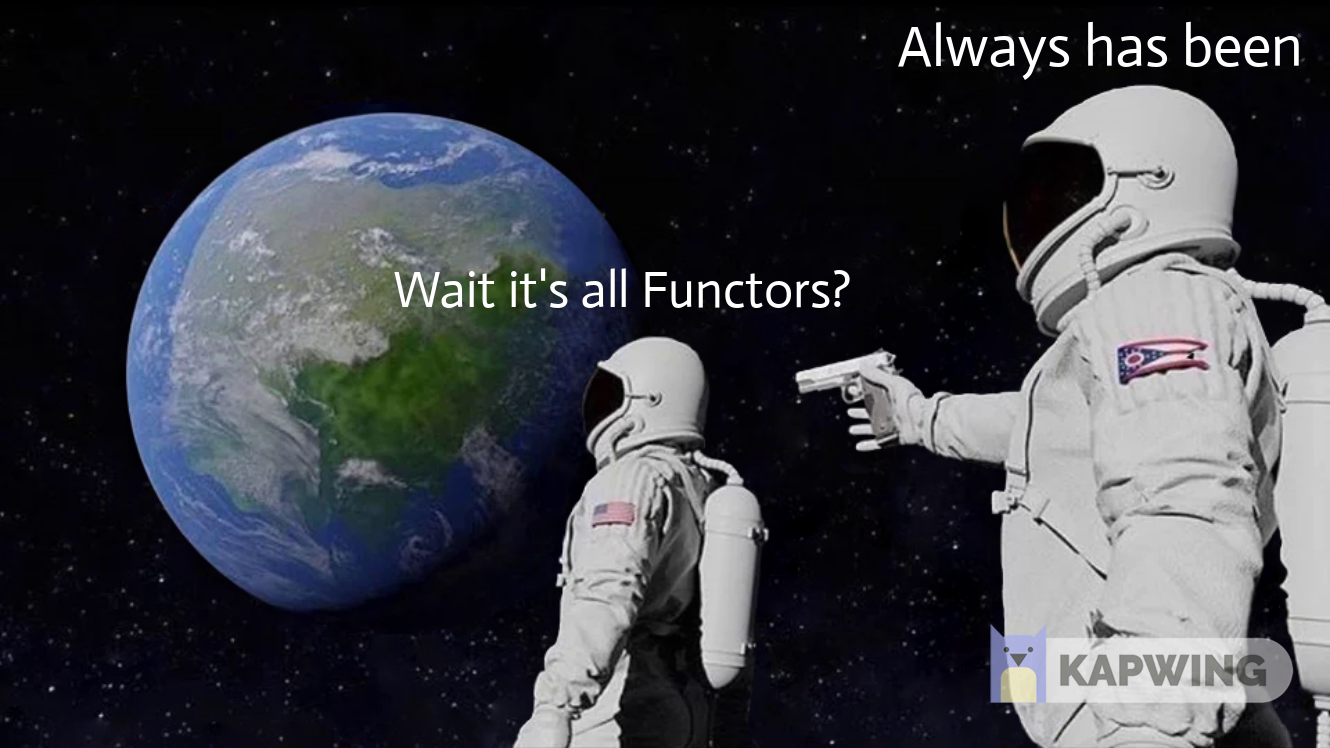
\includegraphics[scale=0.2]{images/astro_meme.png}}
\end{frame}

% Applicatives

\section{Applicatives}

\begin{frame}
    \frametitle{\insertsection}
    \framesubtitle{Red pill, blue pill or purple pill?}
    \centerline{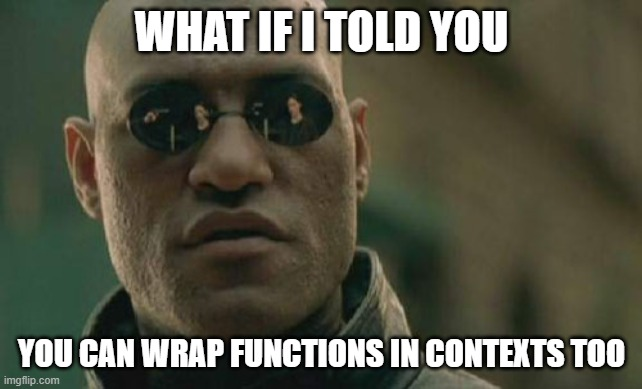
\includegraphics[scale=0.5]{images/what_if.jpg}}
\end{frame}

\begin{frame}
    \frametitle{\insertsection}
    \framesubtitle{Red pill it is\textellipsis}
    \centerline{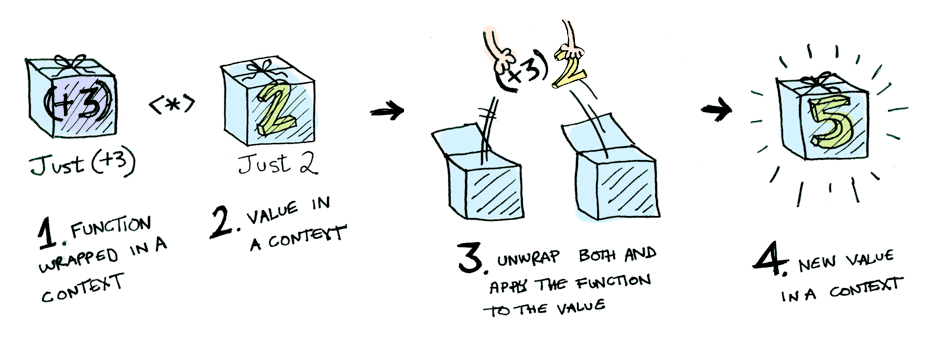
\includegraphics[scale=0.35]{images/applicative_just.png}}
\end{frame}

% Refactoring

\section{Point-free code}

\begin{frame}
    \frametitle{\insertsection}
    \framesubtitle{In the land of the free\textellipsis}
    \centerline{\texttt{f x = 1 + x} vs. \texttt{f = (1+)}}
\end{frame}

\begin{frame}
    \frametitle{\insertsection}
    \framesubtitle{Eta conversion}
    \centerline{
        \texttt{f x = g x}
        }
    \centerline{
        \texttt{f = g}
    }
\end{frame}

\begin{frame}
    \frametitle{\insertsection}
    \framesubtitle{Operator sectioning}

    \centerline{
        \texttt{x + y = (+) x y}
    }
    \centerline{
        \texttt{x + y = ((+) x) y}
    }
    \centerline{
        \texttt{x + y = (x+) y}
    }
\end{frame}

\begin{frame}
    \frametitle{\insertsection}
    \framesubtitle{Composition}
    \centerline{
        \texttt{(f . g) x = f (g x)}
    }
\end{frame}

\section{Bibliography}

\begin{frame}
    \frametitle{\insertsection}
    \nocite{*}
    \printbibliography
\end{frame}

\end{document}
